\documentclass{classrep}
\usepackage[utf8]{inputenc}
\usepackage{color}
\usepackage{enumitem}
\usepackage{graphicx}
\usepackage{amsmath}
\usepackage{float}
\usepackage{hyperref}

\studycycle{Informatyka, studia dzienne, I st.}
\coursesemester{VI}

\coursename{Komputerowe systemy rozpoznawania}
\courseyear{2019/2020}

\courseteacher{dr hab. inż. Adam Niewiadomski prof. uczelni}
\coursegroup{pon., 12:15}

\author{
\studentinfo{Mateusz Walczak}{216911} \and
\studentinfo{Konrad Kajszczak}{216790}
}

\title{Zadanie 2: Lingwistyczne podsumowania baz danych}
\svnurl{https://github.com/Walducha1908/KSR2}

\begin{document}
\maketitle

\section{Cel}
\textit{Praca w toku}


\section{Wprowadzenie}
\textit{Praca w toku}


\section{Opis implementacji}
\textit{Praca w toku}


\section{Materiały i metody}
Wybrana przez nas baza danych zawiera historyczne pomiary pogodowe z Holandii \cite{baza}. Dane zostały zgromadzone przez KNMI (\textit{Dutch weather institute} - Holenderski instytut pogodowy) na przestrzeni lat 1901-2018 i pochodziły z 50 różnych stacji pogowych znajdujących się na terenie całego kraju.\newline

Ze względu na fakt, iż oryginalna baza danych składa się z 804099 krotek, postanowiliśmy wybrać tylko niewielką część z dostępnych danych. Zdecydowaliśmy się na najnowsze dane pomiarowe - z lat 2016-2018. W ten sposób ograniczyliśmy liczbę wykorzystywanych krotek do 17000.\newline

\subsection{Wybór kolumn}
W celu analizy bazy danych i tworzenia jej lingwistycznych podsumowań wybraliśmy następujące 10 kolumn z danymi liczbowymi:

\begin{itemize}[label=$\bullet$\scshape\bfseries]
\item FG - średnia prędkość wiatru przez cały dzień [$0.1 \frac{m}{s}$].
\item FHX - najwyższa średnia prędkość wiatru w ciągu jednej godziny [$0.1 \frac{m}{s}$].
\item FHN - najniższa średnia prędkość wiatru w ciągu jednej godziny [$0.1 \frac{m}{s}$].
\item FXX - najszybszy podmuch wiatru w ciągu całego dnia [$0.1 \frac{m}{s}$].
\item TG - średnia dzienna temperatura [$0.1^{\circ} C$].
\item TN - minimalna dzienna temperatura [$0.1^{\circ} C$].
\item TX - maksymalna dzienna temperatura [$0.1^{\circ} C$].
\item T10N - minimalna dzienna temperatura na wysokości 10 cm od poziomu gruntu [$0.1^{\circ} C$].
\item Q - nasłonecznienie, energia słoneczna przypadająca na powierzchnię [$\frac{J}{cm^2}$].
\item RH - suma opadów atmosferycznych w ciągu całegi dnia [$0.1 mm$].\newline
\end{itemize}

Oprócz wyżej opisanych danych liczbowych, w naszej bazie znajdują się także dwie dodatkowe kolumny, służące do identyfikacji pomiaru:
\begin{itemize}[label=$\bullet$\scshape\bfseries]
\item STN - numer stacji badawczej wykonującej pomiar.
\item YYYYMMDD - data pomiaru w formacie opisanym przez nazwę kolumny.
\end{itemize}

\begin{figure}[H]
	\centering
	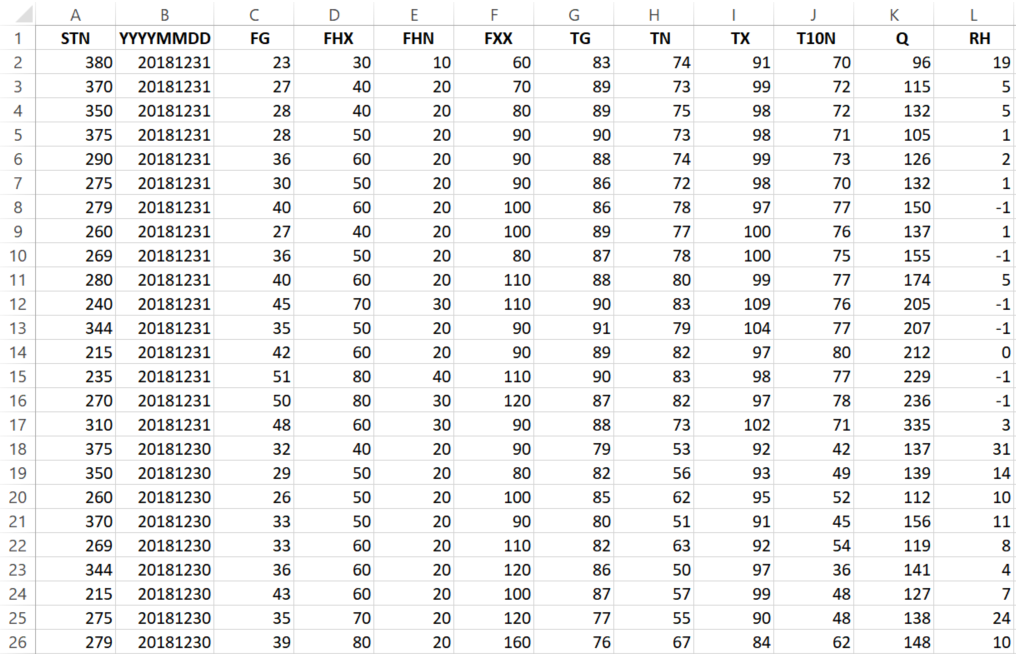
\includegraphics[width=1\textwidth]{Pictures/baza.png}
	\caption{Fragment widoku bazy w formacie $xlsx$}
\end{figure}






\subsection{Przykładowe zmienne lingwistyczne}
W tym rozdziale przedstawimy wzory i wykresy opisujące zaproponowane przez nas zmiennie lingwistyczne. We wszystkich przypadkach, wykorzystywanymi przez nas funkcjami przynależności są funkcje trapezoidalne.  \footnote{Wartości prezentowane w tabelach są tylko propozycjami. Autorzy sprawozdania zastrzegają sobie możliwość do ich późniejszej modyfikacji}.



\subsubsection{Kolumna FG}
Wykres opisujący zmienną lingwistyczną dla kolumny zawierającej wartości średniej prędkości wiatru przez cały dzień (FG), zamieszczono poniżej.
\begin{figure}[H]
	\centering
	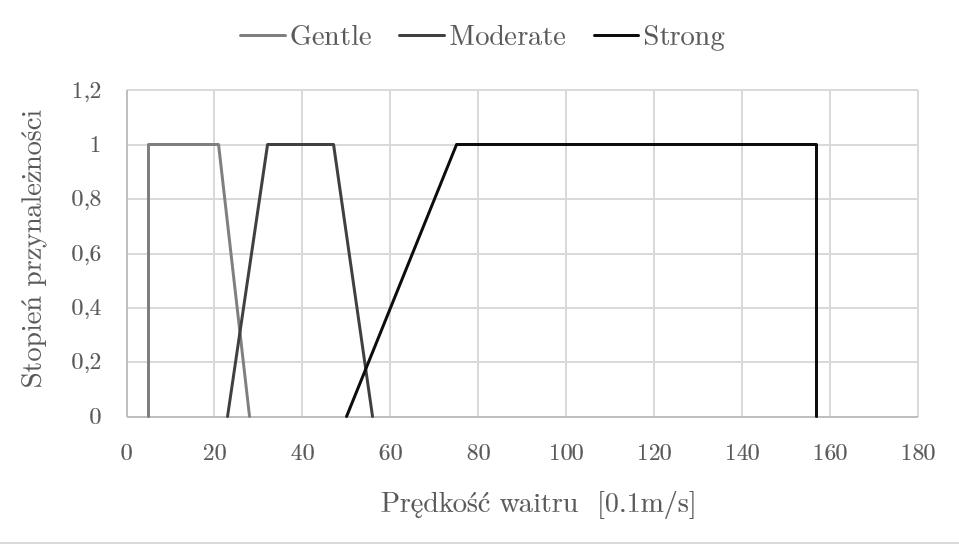
\includegraphics[width=1\textwidth]{Pictures/TermsCharts/FG.png}
	\caption{Wykres opisujący zmienną lingwistyczną dla kolumny FG.}
\end{figure}

Wzory opisujące przynależność do poszczególnych etykiet prezentują się następująco. \newline

Dla etykiety $Gentle$:
\begin{equation}
{FG}_{GENTLE}(x)= \left\{ \begin{array}{ll}
\frac{x-5}{5} 	& \textrm{jeśli $5 \leq x < 10$} \\
1 			& \textrm{jeśli $10 \leq x \leq 21$} \\
\frac{28-x}{7} 	& \textrm{jeśli $21 < x \leq 28$}
\end{array} \right.
\end{equation}

Dla etykiety $Moderate$:
\begin{equation}
{FG}_{MODERATE}(x)= \left\{ \begin{array}{ll}
\frac{x-23}{9} 	& \textrm{jeśli $23 \leq x < 32$} \\
1 			& \textrm{jeśli $32 \leq x \leq 47$} \\
\frac{56-x}{9} 	& \textrm{jeśli $47 < x \leq 56$}
\end{array} \right.
\end{equation}

Dla etykiety $Strong$:
\begin{equation}
{FG}_{STRONG}(x)= \left\{ \begin{array}{ll}
\frac{x-50}{25} 	 & \textrm{jeśli $50 \leq x < 75$} \\
1 			 & \textrm{jeśli $75 \leq x \leq 125$} \\
\frac{157-x}{34} & \textrm{jeśli $125 < x \leq 157$}
\end{array} \right.
\end{equation}



\subsubsection{Kolumna TG}
W przypadku średniej dziennej temperatury (TG), zdecydowaliśmy się podzielić nasze rozważania ze względu na pory roku. Dlatego też przyjęliśmy trzy różne warianty zmiennej lingiwstycznej dla kolumny TG:

\begin{itemize}[label=$\bullet$\scshape\bfseries]
\item TGW - dla pomiarów uzyskanych podczas astronomicznej zimy (litera $W$ od $Winter$),
\item TGSA - dla pomiarów uzyskanych podczas astronomicznej wiosny lub jesieni ($S$ od $Spring$, $A$ od $Autumn$),
\item TGS -dla pomiarów uzyskanych podczas astronomicznego lata  (litera $S$ od $Summer$).
\end{itemize}

Rozpocznijmy od zmiennej lingwistycznej TGW.
\begin{figure}[H]
	\centering
	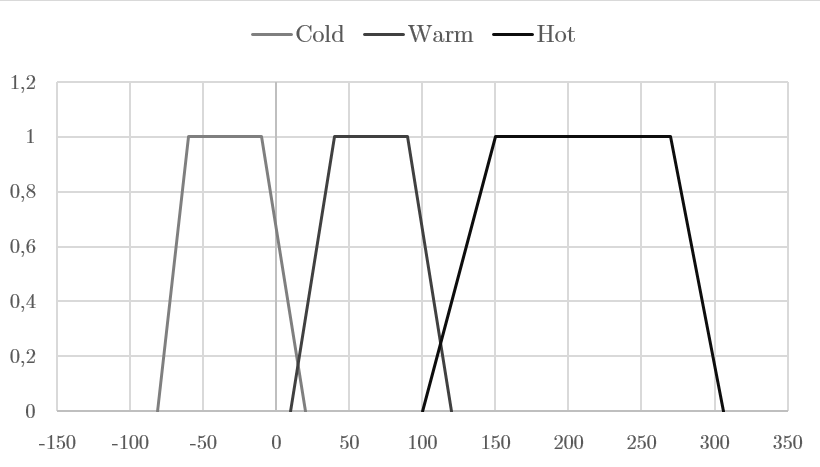
\includegraphics[width=1\textwidth]{Pictures/TermsCharts/TG_Z.png}
	\caption{Wykres opisujący zmienną lingwistyczną dla kolumny TG dla pomiarów wykonanych astronomiczną zimą.}
\end{figure}

Wzory opisujące przynależność do poszczególnych etykiet zmiennej lingwistycznej TGW prezentują się następująco. \newline

Dla etykiety $Cold$:
\begin{equation}
{TGW}_{COLD}(x)= \left\{ \begin{array}{ll}
\frac{x+81}{21} & \textrm{jeśli $-81 \leq x < -60$} \\
1 			& \textrm{jeśli $-60 \leq x \leq -10$} \\
\frac{20-x}{30} 	& \textrm{jeśli $-10 < x \leq 20$}
\end{array} \right.
\end{equation}

Dla etykiety $Warm$:
\begin{equation}
{TGW}_{WARM}(x)= \left\{ \begin{array}{ll}
\frac{x-10}{30} 	 & \textrm{jeśli $10 \leq x < 40$} \\
1 			 & \textrm{jeśli $40 \leq x \leq 90$} \\
\frac{120-x}{30} & \textrm{jeśli $90 < x \leq 120$}
\end{array} \right.
\end{equation}

Dla etykiety $Hot$:
\begin{equation}
{TGW}_{HOT}(x)= \left\{ \begin{array}{ll}
\frac{x-100}{50} & \textrm{jeśli $100 \leq x < 150$} \\
1 			 & \textrm{jeśli $150 \leq x \leq 270$} \\
\frac{306-x}{36} & \textrm{jeśli $270 < x \leq 306$}
\end{array} \right.
\end{equation}

Następną prezentowaną zmienną, będzie zmienna lingwistyczna TGSA.
\begin{figure}[H]
	\centering
	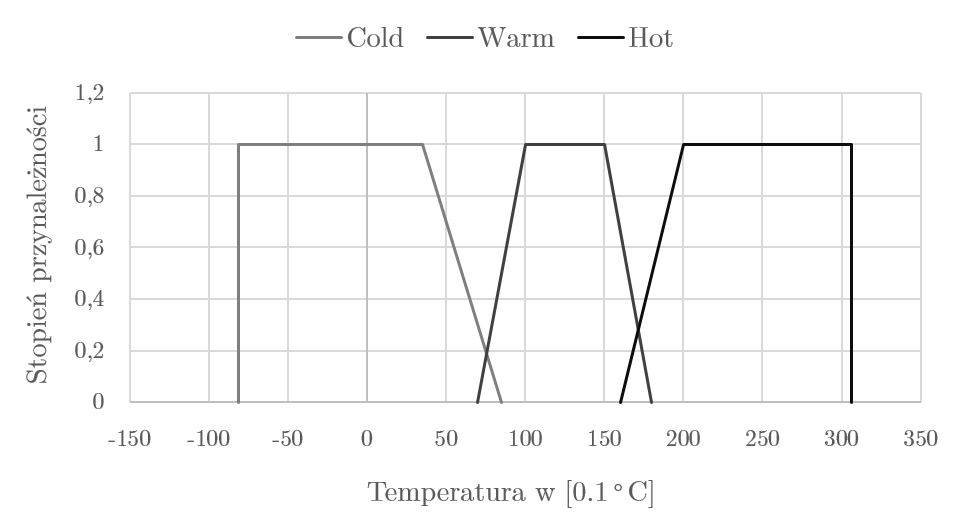
\includegraphics[width=1\textwidth]{Pictures/TermsCharts/TG_WJ.png}
	\caption{Wykres opisujący zmienną lingwistyczną dla kolumny TG dla pomiarów wykonanych astronomiczną wiosną i jesienią.}
\end{figure}

Wzory opisujące przynależność do poszczególnych etykiet zmiennej lingwistycznej TGSA prezentują się następująco. \newline

Dla etykiety $Cold$:
\begin{equation}
{TGSA}_{COLD}(x)= \left\{ \begin{array}{ll}
\frac{x+81}{31} & \textrm{jeśli $-81 \leq x < -50$} \\
1 			& \textrm{jeśli $-50 \leq x \leq 35$} \\
\frac{85-x}{50} 	& \textrm{jeśli $35 < x \leq 85$}
\end{array} \right.
\end{equation}

Dla etykiety $Warm$:
\begin{equation}
{TGSA}_{WARM}(x)= \left\{ \begin{array}{ll}
\frac{x-70}{30} 	 & \textrm{jeśli $70 \leq x < 100$} \\
1 			 & \textrm{jeśli $100 \leq x \leq 150$} \\
\frac{180-x}{30} & \textrm{jeśli $150 < x \leq 180$}
\end{array} \right.
\end{equation}

Dla etykiety $Hot$:
\begin{equation}
{TGSA}_{HOT}(x)= \left\{ \begin{array}{ll}
\frac{x-160}{40} & \textrm{jeśli $160 \leq x < 200$} \\
1 			 & \textrm{jeśli $200 \leq x \leq 270$} \\
\frac{306-x}{36} & \textrm{jeśli $270 < x \leq 306$}
\end{array} \right.
\end{equation}\newline

Ostatnią zmienną dla kolumny TG będzie zmienna dotycząca pomiarów letnich - TGS.
\begin{figure}[H]
	\centering
	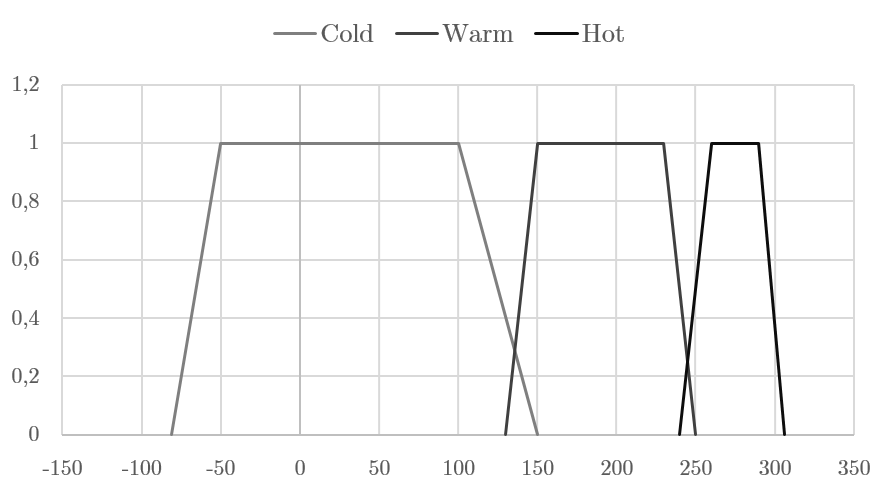
\includegraphics[width=1\textwidth]{Pictures/TermsCharts/TG_L.png}
	\caption{Wykres opisujący zmienną lingwistyczną dla kolumny TG dla pomiarów wykonanych astronomicznym latem.}
\end{figure}

Wzory opisujące przynależność do poszczególnych etykiet zmiennej lingwistycznej TGS prezentują się następująco. \newline

Dla etykiety $Cold$:
\begin{equation}
{TGS}_{COLD}(x)= \left\{ \begin{array}{ll}
\frac{x+81}{31} & \textrm{jeśli $-81 \leq x < -50$} \\
1 			& \textrm{jeśli $-50 \leq x \leq 100$} \\
\frac{150-x}{50}& \textrm{jeśli $100 < x \leq 150$}
\end{array} \right.
\end{equation}

Dla etykiety $Warm$:
\begin{equation}
{TGS}_{WARM}(x)= \left\{ \begin{array}{ll}
\frac{x-130}{20} & \textrm{jeśli $130 \leq x < 150$} \\
1 			 & \textrm{jeśli $150 \leq x \leq 230$} \\
\frac{250-x}{20} & \textrm{jeśli $230 < x \leq 250$}
\end{array} \right.
\end{equation}

Dla etykiety $Hot$:
\begin{equation}
{TGS}_{HOT}(x)= \left\{ \begin{array}{ll}
\frac{x-240}{20} & \textrm{jeśli $240 \leq x < 260$} \\
1 			 & \textrm{jeśli $260 \leq x \leq 290$} \\
\frac{306-x}{16} & \textrm{jeśli $290 < x \leq 306$}
\end{array} \right.
\end{equation}




\subsubsection{Kolumna Q}
Wykres opisujący zmienną lingwistyczną dla kolumny zawierającej wartości nasłonecznienia (Q), zamieszczono poniżej.
\begin{figure}[H]
	\centering
	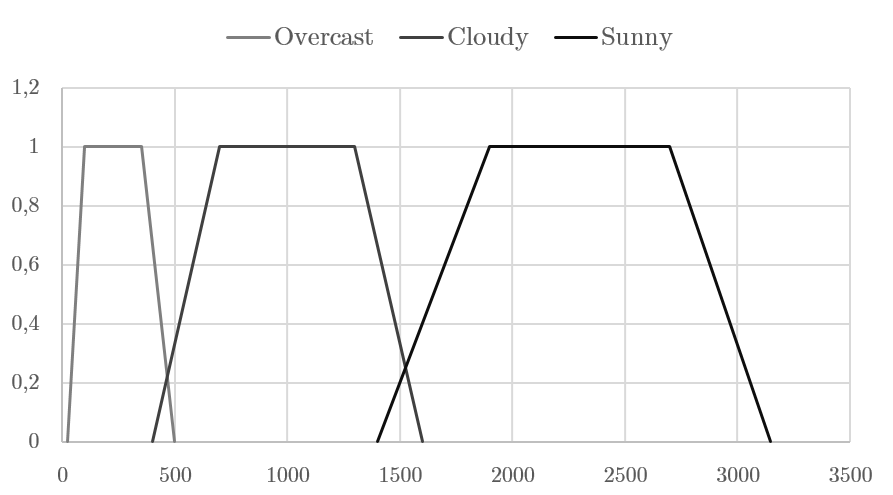
\includegraphics[width=1\textwidth]{Pictures/TermsCharts/Q.png}
	\caption{Wykres opisujący zmienną lingwistyczną dla kolumny Q}
\end{figure}

Wzory opisujące przynależność do poszczególnych etykiet zmiennej lingwistycznej Q prezentują się następująco. \newline

Dla etykiety $Overcast$:
\begin{equation}
{Q}_{OVERCAST}(x)= \left\{ \begin{array}{ll}
\frac{x-24}{76} & \textrm{jeśli $24 \leq x < 100$} \\
1 			& \textrm{jeśli $100 \leq x \leq 350$} \\
\frac{500-x}{150}& \textrm{jeśli $350 < x \leq 500$}
\end{array} \right.
\end{equation}

Dla etykiety $Cloudy$:
\begin{equation}
{Q}_{CLOUDY}(x)= \left\{ \begin{array}{ll}
\frac{x-400}{300} & \textrm{jeśli $400 \leq x < 700$} \\
1 			 & \textrm{jeśli $700 \leq x \leq 1300$} \\
\frac{1600-x}{300} & \textrm{jeśli $1300 < x \leq 1600$}
\end{array} \right.
\end{equation}

Dla etykiety $Sunny$:
\begin{equation}
{Q}_{SUNNY}(x)= \left\{ \begin{array}{ll}
\frac{x-1400}{500} & \textrm{jeśli $1400 \leq x < 1900$} \\
1 			 & \textrm{jeśli $1900 \leq x \leq 2700$} \\
\frac{3145-x}{445} & \textrm{jeśli $2700 < x \leq 3145$}
\end{array} \right.
\end{equation}



\section{Wyniki}
\textit{Praca w toku}


\section{Dyskusja}
\textit{Praca w toku}


\section{Wnioski}
\textit{Praca w toku}


\begin{thebibliography}{1}
\bibitem{baza} 
Baza danych - 
\href{https://www.kaggle.com/sinaasappel/historical-weather-in-the-netherlands-19012018}{\textit{"Historical weather in the Netherlands 1901-2018"}}
\end{thebibliography}
\end{document}
